% This file was created by tikzplotlib v0.9.8.
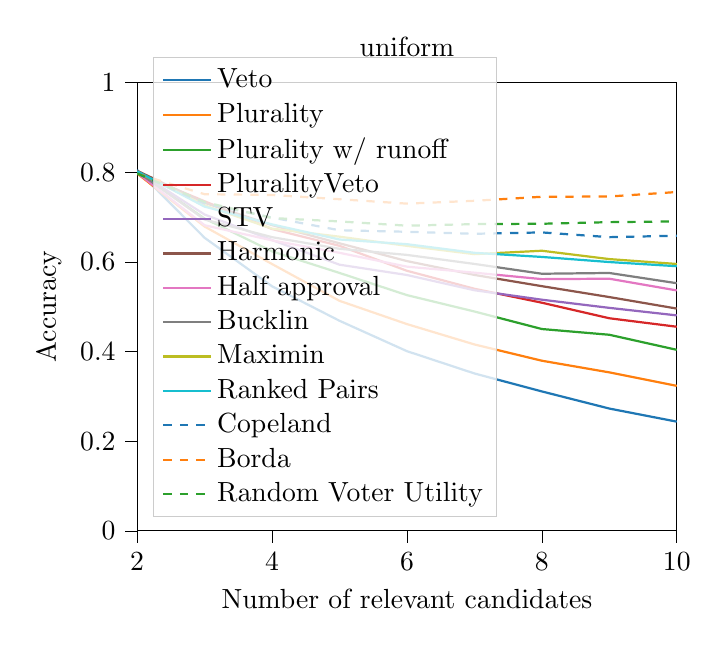
\begin{tikzpicture}

\definecolor{color0}{rgb}{0.12156862745098,0.466666666666667,0.705882352941177}
\definecolor{color1}{rgb}{1,0.498039215686275,0.0549019607843137}
\definecolor{color2}{rgb}{0.172549019607843,0.627450980392157,0.172549019607843}
\definecolor{color3}{rgb}{0.83921568627451,0.152941176470588,0.156862745098039}
\definecolor{color4}{rgb}{0.580392156862745,0.403921568627451,0.741176470588235}
\definecolor{color5}{rgb}{0.549019607843137,0.337254901960784,0.294117647058824}
\definecolor{color6}{rgb}{0.890196078431372,0.466666666666667,0.76078431372549}
\definecolor{color7}{rgb}{0.737254901960784,0.741176470588235,0.133333333333333}
\definecolor{color8}{rgb}{0.0901960784313725,0.745098039215686,0.811764705882353}

\begin{axis}[
legend cell align={left},
legend style={
  fill opacity=0.8,
  draw opacity=1,
  text opacity=1,
  at={(0.03,0.03)},
  anchor=south west,
  draw=white!80!black
},
tick align=outside,
tick pos=left,
title={uniform},
x grid style={white!69.0196078431373!black},
xlabel={Number of relevant candidates},
xmin=2, xmax=10,
xtick style={color=black},
y grid style={white!69.0196078431373!black},
ylabel={Accuracy},
ymin=0, ymax=1,
ytick style={color=black}
]
\addplot [thick, color0]
table {%
2 0.8049
3 0.6536
4 0.5454
5 0.4685
6 0.4007
7 0.351
8 0.3109
9 0.2727
10 0.2435
};
\addlegendentry{Veto}
\addplot [thick, color1]
table {%
2 0.7972
3 0.6787
4 0.595
5 0.513
6 0.4611
7 0.4157
8 0.3794
9 0.3534
10 0.3233
};
\addlegendentry{Plurality}
\addplot [thick, color2]
table {%
2 0.8014
3 0.6965
4 0.6233
5 0.5752
6 0.5257
7 0.4892
8 0.4501
9 0.4373
10 0.4037
};
\addlegendentry{Plurality w/ runoff}
\addplot [thick, color3]
table {%
2 0.7974
3 0.7351
4 0.6731
5 0.6357
6 0.58
7 0.5399
8 0.5088
9 0.4741
10 0.4552
};
\addlegendentry{PluralityVeto}
\addplot [thick, color4]
table {%
2 0.8017
3 0.7055
4 0.6485
5 0.5936
6 0.5706
7 0.5366
8 0.5155
9 0.4973
10 0.4805
};
\addlegendentry{STV}
\addplot [thick, color5]
table {%
2 0.8031
3 0.7316
4 0.6819
5 0.6413
6 0.6016
7 0.5708
8 0.5457
9 0.5214
10 0.4957
};
\addlegendentry{Harmonic}
\addplot [thick, color6]
table {%
2 0.7986
3 0.6816
4 0.6478
5 0.6201
6 0.5892
7 0.5758
8 0.5614
9 0.5623
10 0.5362
};
\addlegendentry{Half approval}
\addplot [thick, white!49.8039215686275!black]
table {%
2 0.8015
3 0.6944
4 0.655
5 0.6291
6 0.6154
7 0.5953
8 0.5734
9 0.5751
10 0.5523
};
\addlegendentry{Bucklin}
\addplot [thick, color7]
table {%
2 0.8003
3 0.726
4 0.6741
5 0.6561
6 0.6356
7 0.6171
8 0.6247
9 0.6061
10 0.5952
};
\addlegendentry{Maximin}
\addplot [thick, color8]
table {%
2 0.8019
3 0.7231
4 0.6835
5 0.6498
6 0.6393
7 0.6201
8 0.6109
9 0.5995
10 0.5902
};
\addlegendentry{Ranked Pairs}
\addplot [thick, color0, dashed]
table {%
2 0.797
3 0.7304
4 0.6987
5 0.6704
6 0.667
7 0.6625
8 0.6656
9 0.655
10 0.6582
};
\addlegendentry{Copeland}
\addplot [thick, color1, dashed]
table {%
2 0.7963
3 0.7508
4 0.7491
5 0.7396
6 0.7298
7 0.7361
8 0.7451
9 0.7457
10 0.7557
};
\addlegendentry{Borda}
\addplot [thick, color2, dashed]
table {%
2 0.7971
3 0.7333
4 0.6977
5 0.6901
6 0.6806
7 0.6841
8 0.6849
9 0.6885
10 0.6901
};
\addlegendentry{Random Voter Utility}
\end{axis}

\end{tikzpicture}
